
\section{Greedy and approximation algorithms}


\subsection{An activity-selection problem}
\begin{tabular}{m{6cm}m{10cm}}
    Find the max number of activities that do not
    overlap in time : 
    $$\forall i,j \quad selected: \quad s_i \geq f_j  \quad or \quad s_j \geq f_i$$
    &
\begin{itemize}
    \item $s_i$ = start time of activity
    \item $f_i$ = end time activity (not that activities are 
        sorted such that $f_i \leq f_{i+1}$)
\end{itemize}
\end{tabular}

\begin{enumerate}
    \item \textbf{Reduction} to the maximum independent set problem where 
        we find the maximum set of vertices in a graph such that
        to vertices selected are not adjacent.

        \begin{tabular}{m{10cm}m{3cm}}
            \begin{itemize}
                \item The reduction is done by add an edge between $i$ and $j$ if
                    activities overlap in time: 
                    $$s_i < f_j and s_j < f_i$$ 
            \end{itemize}
            Note that the maximum independent set problem is NP-Hard problem
            &
            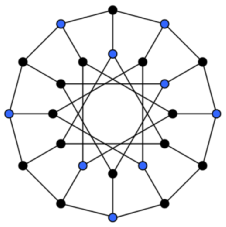
\includegraphics[width=3cm]{img/independant}
        \end{tabular}


    \item \textbf{Dynamic programming}: select a maximum size subset of mutually
        compatible activities from $S_{ij}$, for $0 \leq i < j \leq n+1$,
        knowing that all other $S_{ij}$ are empty.

        $a_m$ such that $f_m = min\{f_k: a_k \in S_{ij}\}$
        \[
            c[i, j] = 
            \begin{cases} 
                0 & \text{if } S_{ij} = \emptyset \\
                max_{\substack{i<k<j \\ a_k \in S_{ij}}} \{c[i, k] + c[k, j] + 1\}  & \text{if } S_{ij} \neq \emptyset
            \end{cases}
        \]
        \begin{itemize}
                %TODO
            \item Time complexity: 
            \item Space complexity: 
        \end{itemize}

        \paragraph{Improvement to a greedy}
        \begin{itemize}
            \item Obs.1: a m is used in some maximum-size subset of
                mutually compatible activities of $S_ij$

                Proof (Sketch):
                \begin{small}
                    Suppose $A_{ij}$ an optimal set of $S_{ij}$ . Take
                    the first activity of $A_{ij}$ (assume it is $a_k$ with $k \neq m$). We
                    can safely replace $a_k$ with $a_m$ because $f_m \leq f_k$.
                \end{small}

            \item Obs.2: The subproblem $S_im$ is empty, so that choosing
                $a_m$ (in the recurrence) leaves the subproblem $S_mj$ as the
                only one that may be nonempty.
        \end{itemize}

        %TODO new recurrence equation

    \item \textbf{Greedy algorithm}
        \begin{lstlisting}[mathescape]
n $=$ nbrActivities
A $= a_1$
i $= 1$

for m $\leftarrow$ 2 to n do
if $s_m \geq f_i$ then
A = $A \cup a_m$
i =$m$

return A
        \end{lstlisting}
\end{enumerate}


\subsection{Greedy}
At each decision point, the algorithm makes
a \textbf{local optimum choice} in the hope that it is a global
optimum choice.
\begin{itemize}
    \item For some problem it's the case
    \item For other it's not and sometimes we can 
        have a guarantee how
        \textit{suboptimal} we can be.
\end{itemize}


\subsection{Minimum Spanning Tree (MST)}

\subsubsection{Definition}
\begin{itemize}
    \item A \textbf{cut} (S,V-S) of an undirected graph
    \item An edge (u,v) \textbf{cross} the cut (S,V-S) if one of its
        endpoints is in S and the other in V-S
    \item A cut \textbf{respects} a set A of edges if no edge in A crosses
        the cut.
    \item An edge is a \textbf{light edge} crossing a cut if its weight is
        the minimum of any edge crossing the cut. (can be
        more than one in case of ties).
\end{itemize}

\subsubsection{Theorem}
\begin{itemize}
    \item[LET]
    \item $G=(V,E)$ a undirected graph with weight function $w$ on $E$.
    \item $A \subseteq E$ included in some MST for $G$.
    \item $(S, V-S)$ be any cut of $G$ that respect $A$
    \item $(u,v)$ be a light edge crossing $(S, V-S)$
    \item[THEN]
    \item edge $(u, v)$ is safe for $A$
\end{itemize}

\paragraph{Proof}
Let $T$ be a minimum spanning tree that includes $A$, and assume
that $T$ does not contain the light edge $(u,v)$, since if it does we
are done.

\begin{enumerate}
    \item Because $(u,v)$ are on opposite sides
        of the cut $(S,V-T)$ that respects $A$,
        there is necessarily some edge $(x,y)$
        on path $p$ also on opposite sides of
        the cut.

    \item We can form an other MST $T'$ by
        removing $(x,y)$ and adding $(u,v)$ from
        $T$. Because when considering $A$,
        $(u,v)$ is a light edge, $(x,y)$ cannot be
        cheaper than $(u,v)$ (by definition of a
        light edge).
\end{enumerate}


\subsubsection{Algorithm}

\begin{lstlisting}[mathescape, caption=Generic-MST(V\,E\,c\,s\,t)]
A = $\emptyset$
while A does not form a spanning tree do
    find an edge $(u, v)$ that is safe for A
    A = A $\cup \{(u, v)\}$

return A
\end{lstlisting}

\begin{itemize}
    \item \textbf{Kruskal}  
        
        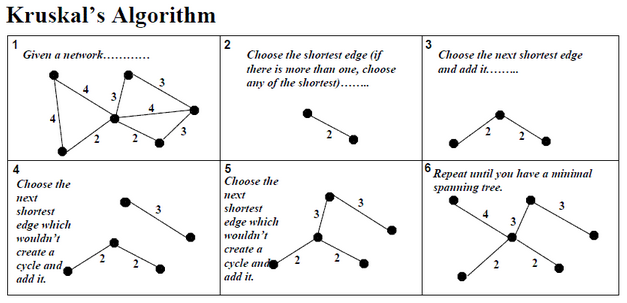
\includegraphics[width=14cm]{img/kruskalAlgo}
    \item \textbf{Prim} 
        
        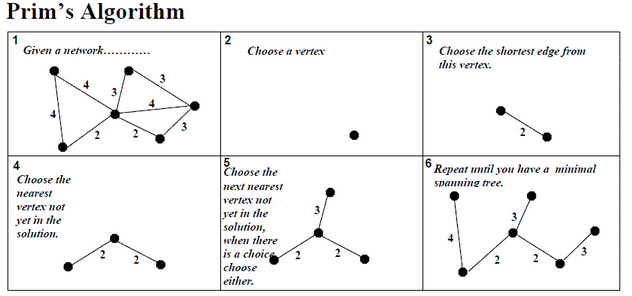
\includegraphics[width=14cm]{img/primAlgo}
\end{itemize}

\subsubsection{Implementation using disjoint-set forests}
Kruskal and prim can be implemented in $O(E \times log(V))$

\begin{lstlisting}[mathescape, caption=MST-Kruskal(G\,w)]
A = $\emptyset$
for each vertex $v \in V$ do
    Make-Set-(v)

sort the edge of $E$ into non decreasing order by weight $w$
for each edge $(u,v) \in E$ taken in non decreasing order by weight do
    if Find-Set(u) $\neq$ Find-Set(v) then
        A = A $\cup \{(u, v)\}$
        Union(u,v)

return A
\end{lstlisting}

\begin{center}
\begin{tabular}{m{7cm}m{7cm}}
    \begin{lstlisting}[mathescape]
MAKE-SET(x)
    X.p = x
    x.rank = 0

FIND-SET(x)
    if x $\neq$ x.p
        x.p = fIND-SET(x.p)
    return x.p
    \end{lstlisting}
    &
    \begin{lstlisting}[mathescape]
UNION(x, y)
    LINK(FIND-SET(x), FIND-SET(y))

LINK(x, y)
    if x.rank > y.rank
        y.p = x
    else 
        x.p = y
        if x.rank == y.rank
            y.rank = y.rank + 1
    \end{lstlisting}\\
    $\rightarrow$ Path compression
    & 
    $\rightarrow$ Union by rank
\end{tabular}
\end{center}

\begin{itemize}
    \item \texttt{Sort} in $O(E \times log(E)) = O(E \times log(V^2)) = O(E \times log(V))$
    \item \texttt{Make-Set(x)}: make a set with $x$
    \item \texttt{Find-Set(x)}: return pointer to the set containing $x$

        \paragraph{O(1)} is assured by using \textbf{path compression}.

        \begin{tabular}{m{11cm}m{3cm}}
            During Find-Set operation, make each node
            on the find path point directly to the root
            &
            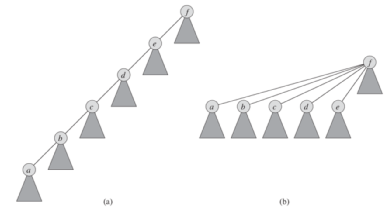
\includegraphics[width=3cm]{img/compression}
    \end{tabular}


    \item \texttt{Union(x, y)}: merge two sets (can't have a duplicate element
        because of set)

        \paragraph{O(1)} is assured by using \textbf{union by rank}.

        \begin{tabular}{m{11cm}m{3cm}}
            Make the root of the tree with the fewer nodes points to
            the root of the tree with more nodes.
            &
            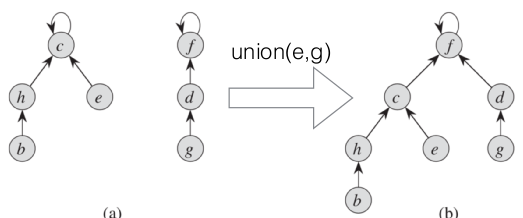
\includegraphics[width=4cm]{img/union}
    \end{tabular}
\end{itemize}

\begin{itemize}
    \item The time complexity of $m$ (> n) operations on $n$ objects
        using Disjoint-set forests implemented with path
        compression and union by rank $i$: 
        $$\Theta(m \alpha(m,n))$$
    \item $\rightarrow \alpha(m, n)$ is the inverse Ackermann's function. 
        In fact, it's less than 5 for any practical input size $n$
\end{itemize}

\subsection{Approximation}

An algorithm for a problem has an \textbf{approximation ratio} of $\rho(n)$ if
for any input size $n$, the cost $C$ of the solution is within a factor
$\rho(n)$ of the cost C* of an optimal solution.
$$max(\frac{C}{C*}, \frac{C*}{C}) \leq \rho(n)$$

\subsubsection{Set cover example}
Minimum set of vertices such that each
edge of the graph is incident to at least one vertex of
the set.

\begin{lstlisting}[mathescape, caption=Greddy set cover]
C = $\emptyset$
E' = G.E
while E' $\neq \emptyset$ do
    $(u, v)$ be arbitrary edge of E'
    C = C $\cup \{u, v\}$
    remove from E' every edge incident on either $u$ or $v$

return C
\end{lstlisting}

%TODO slide 29 et + lecture 06
TODO slide 29 et + lecture 06

\subsubsection{Subset-sum}

\subsection{Exam}
\begin{itemize}
    \item All theoretical notions introduced (proofs, etc).
    \item Design a greedy algorithm
    \item MST: I give you a new MST greedy algorithm. You
        should be able argument whether it is correct or not.
    \item Design a simple approximation scheme, compute it’s
        approximation ratio
    \item I give you a complexity of an approximation scheme.
        You should be able to tel me if it is fully polynomial.
\end{itemize}
